% Setup - do not change
\documentclass[11pt]{article}
\usepackage[top=0.9in, left=0.9in, bottom=0.9in, right=0.9in]{geometry} 
\usepackage{parskip}

\usepackage[english]{babel}
\usepackage[utf8]{inputenc}
\usepackage{amsmath,amsthm,amssymb,graphicx,pdfpages,lipsum,hyperref}
\usepackage[none]{hyphenat}
\usepackage{csquotes}

\setlength\parindent{0pt}
%%%%%%%%%%%%%%%%%%%%%%%%%%%%%%%%%%%%%%%%%%%%%%%%%%%%%%%%%%%%%%%%%%%
% add other packages here if required

%% Bibliography are specified in this file. You can also choose inline bib style if you want to. But make sure your citation style is consistent (and proper)
% For more details on citation: https://library.unimelb.edu.au/recite
\usepackage[sorting = none]{biblatex}
\addbibresource{references.bib}

%%%%%%%%%%%%%%%%%%%%%%%%%%%%%%%%%%%%%%%%%%%%%%%%%%%%%%%%%%%%%%%%%%% the '%' symbol denotes comments

% Begin document creation
% DELETE THE \lipsum PLACEHOLDERS WHEN YOU BEGIN
\title{\textbf{MAST30034 Project 1} \\ Predicting Profitibality of Taxi Rides in NYC}
\author{
Aarav Nair \\
Student ID: 1287210 \\
%% Replace the link with your github repo
% 1. Remember to escape underscore (\_) in the link.
% 2. Remember to include the commit you want to submit in the link
\href{https://github.com/MAST30034-AppliedDataScience/project-1-individual-tumblesbdj}{Github Repo}
}

\begin{document}
\maketitle 

\section{Introduction} 

As the most populous city in the United States, New York City sees millions of taxi rides each month. This project aims to analyze the New York City Taxi and Limousine Commission (TLC) trip record data\cite{tlc_data}, along with weather data, to develop a model that can accurately predict when a taxi ride will be profitable. By identifying these profitable trips and optimizing routes with predictive analytics—such as using synthetic data generated from weather predictions and historical pickup locations—the model seeks to assist both taxi drivers and the corporations that manage these services in maximizing income and improving operational efficiency.

\section{Data Selection}

For this project, three primary datasets were utilized:

\begin{itemize}
    \item \textbf{New York City Taxi and Limousine Commission (TLC) Trip Record Data:} This dataset contains detailed records of taxi trips in New York City, including information on trip duration, distance, fare amount, and pickup/drop-off locations.

    \item \textbf{Weather Data:} External weather data was integrated to analyze the impact of weather conditions on taxi demand and profitability. This dataset includes variables such as temperature, precipitation, and wind speed.

    \item \textbf{Taxi Zone Data:} This dataset provides the geographical boundaries of taxi zones in New York City, allowing for the spatial analysis of trip data. 
\end{itemize}

\section{Data Preprocessing}

\subsection{Data Cleaning}

To ensure data quality and consistency, several cleaning steps were applied to the dataset:

\begin{itemize}
    \item \textbf{Outlier Detection via IQR:} Outliers were detected and removed in the \texttt{fare\_amount}, \texttt{trip\_distance}, \texttt{trip\_duration}, and \texttt{tip\_amount} columns using a modified Interquartile Range (IQR) method. The lower and upper bounds were calculated based on the formula:
    \[
    \text{Lower Bound} = Q1 - \left(N^{0.5} - 0.5\right) \times IQR
    \]
    \[
    \text{Upper Bound} = Q3 + \left(N^{0.5} - 0.5\right) \times IQR
    \]
    where \( N \) is the number of observations, \( Q1 \) is the first quartile, \( Q3 \) is the third quartile, and \( IQR \) is the interquartile range.

    \item \textbf{Temporal Filtering:} Ensured that all trips occurred within the first six months of the year. Pickup and drop-off datetime values were filtered to remove any records outside the expected range.

    \item \textbf{Passenger Count:} Filtered records to include only those with a passenger count between 1 and 6, as per the legal limit.

    \item \textbf{Geospatial Validity:} Ensured that the Pickup and Dropoff Location IDs were within the valid range [1, 263], corresponding to the NYC taxi zones.

    \item \textbf{Removing Airport Locations:} To avoid trivial observations about the obvious profitability surrounding airports, location IDs 132 and 138 were removed.
\end{itemize}

\subsection{Feature Engineering}

Several new features were engineered to enhance model performance:

\begin{itemize}
    \item \textbf{Profitability:} Profitability was intended to be a measure of the driver's revenue per unit time. As calculated below:
    \[
    \text{Profitability} = \frac{\text{fare\_amount} + \text{extra} + \text{tip\_amount}}{\text{trip\_duration}}
    \]
    This was later categorized into a boolean feature indicating whether a trip was profitable by testing if it was in the top 25\% (75th Quantile) of profitability.

    \item \textbf{Trip Duration:} Calculated from the difference between drop-off and pickup times (in minutes).

    \item \textbf{Temporal Features:} Extracted features such as hour of the day, day of the week, and month from the pickup datetime to capture temporal patterns.

    \item \textbf{Weather Features:} Integrated external weather data, including temperature, precipitation, and wind speed.
\end{itemize}

\subsection{Dropping Irrelevant Columns}

During the preprocessing stage, several columns were identified as irrelevant or redundant and were therefore removed to simplify the dataset and reduce computational complexity. For instance:

\begin{itemize}
    \item \textbf{\texttt{VendorID}:} This column, which indicates the data provider. Not deemed noteworthy.

    \item \textbf{\texttt{store\_and\_fwd\_flag}:} This flag, which indicates whether a trip record was stored in the vehicle's memory before being sent to the server, was also considered irrelevant and was dropped from the dataset.
\end{itemize}

\section{Analysis and Visualization}

In this section, we explore the key insights derived from the data through various visualizations, focusing on the spatial and temporal distribution of taxi trips, their profitability, and the influence of weather conditions on profitability.

\subsection{Spatial Distribution and Profitability of Taxi Pickups}

The spatial analysis of taxi activity in New York City reveals distinct patterns in both the volume of taxi pickups and the profitability of these rides. As illustrated in Figure \ref{fig:pickup_location}, the majority of taxi pickups are concentrated in Manhattan, particularly in the Midtown and Downtown areas, driven by the high density of businesses, tourist attractions, and nightlife in these regions. In contrast, Brooklyn, Queens, and the Bronx show significantly lower taxi pickup volumes, corresponding to their lower population density and fewer commercial activities.

However, when examining the profitability of taxi trips, as shown in Figure \ref{fig:prof_by_location}, a different pattern emerges. While Midtown Manhattan and Downtown areas remain active, the most profitable trips are concentrated in specific areas of Brooklyn and Queens. These areas, despite having fewer pickups, yield higher profitability, likely due to longer trips or higher tips. This contrast highlights that areas with higher taxi demand do not necessarily translate to higher profits.

\begin{figure}[h]
    \centering
    \begin{minipage}{0.48\textwidth}
        \centering
        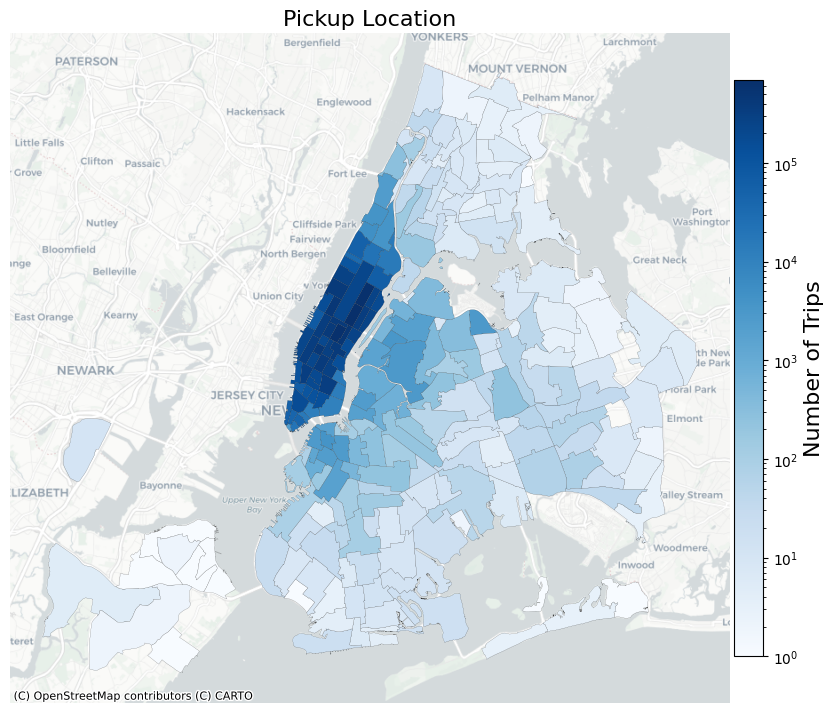
\includegraphics[width=\textwidth]{plots/pickup_frequency_map.png}
        \caption{Spatial distribution of taxi pickups across New York City.}
        \label{fig:pickup_location}
    \end{minipage}\hfill
    \begin{minipage}{0.48\textwidth}
        \centering
        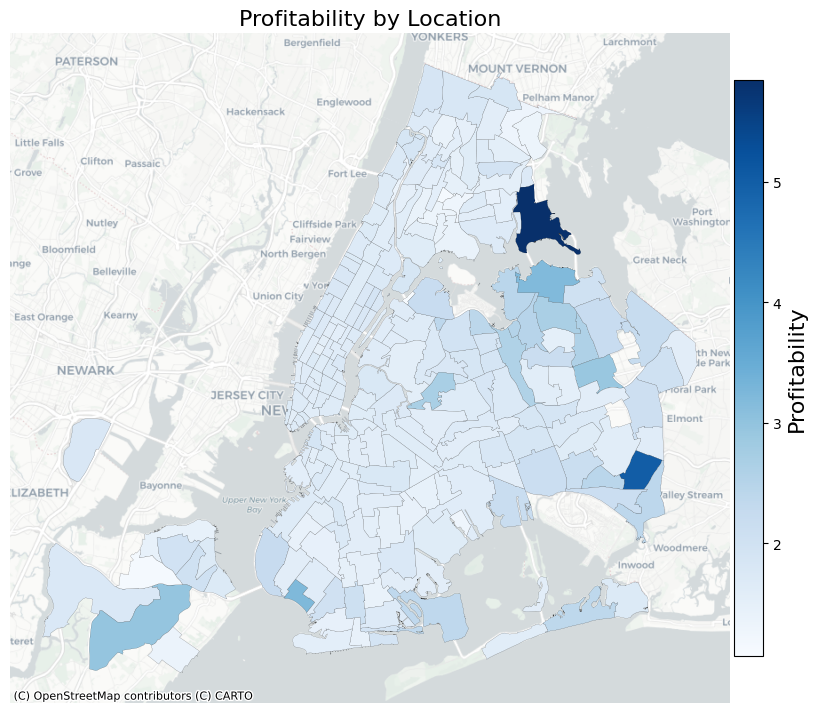
\includegraphics[width=\textwidth]{plots/profbylocation.png}
        \caption{Spatial distribution of taxi trip profitability across New York City.}
        \label{fig:prof_by_location}
    \end{minipage}
\end{figure}

\subsection{Taxi Usage by Hour and Day of the Week}
The heatmap in Figure \ref{fig:usage_day_time} illustrates the pattern of taxi usage across different hours of the day and days of the week. The highest usage is observed during the evening rush hours, particularly from 5 PM to 7 PM on weekdays, which aligns with the time when people are likely commuting home from work. Conversely, the lowest usage occurs in the early morning hours between midnight and 6 AM. The heatmap also shows a noticeable difference between weekdays and weekends, with weekend usage peaking later in the day, likely due to leisure activities.

\pagebreak

\begin{figure}[h]
    \centering
    \vspace{-5mm} % Adjust vertical space
    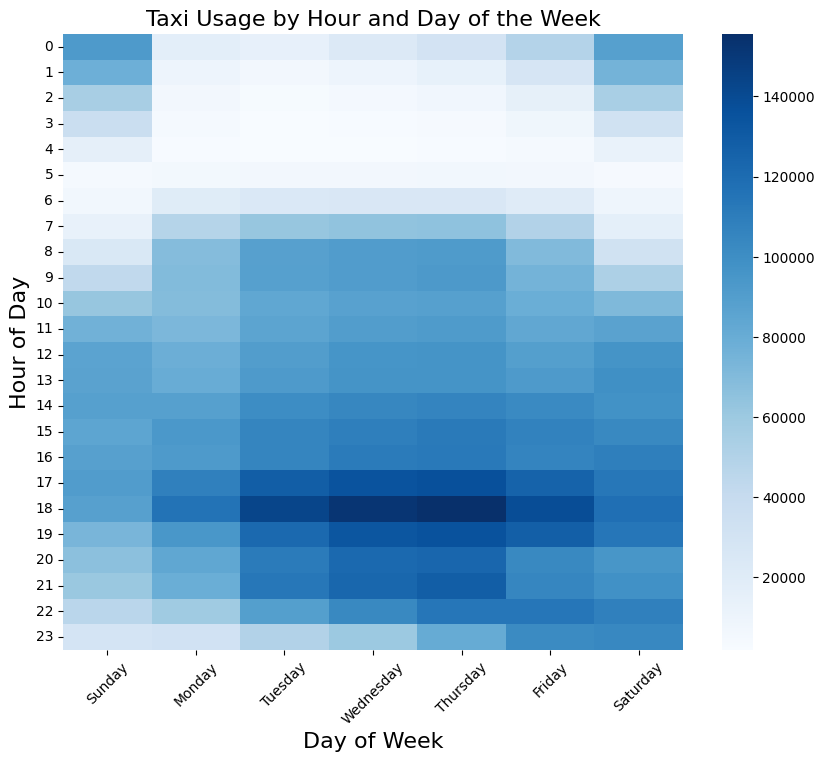
\includegraphics[width=0.45\textwidth]{plots/usage_day_time.png} % Adjusted width for better fit
    \caption{Taxi usage by hour and day of the week in New York City.}
    \label{fig:usage_day_time}
    \vspace{-5mm} % Adjust vertical space
\end{figure}

\subsection{Profitability by Day of Week and Hour of Day}
Figure \ref{fig:profdaytime} illustrates the average profitability of taxi trips across different days of the week and hours of the day. The heatmap reveals that early morning hours, particularly between 4 AM and 6 AM, show higher profitability throughout the week. This might be due to higher fare rates or additional tips during late-night or early morning trips, possibly from airport runs or late-night passengers. Interestingly, while weekdays and weekends both show high profitability in the early morning, weekdays also display a secondary peak in the late afternoon, likely associated with the evening rush hour.

\begin{figure}[h]
    \centering
    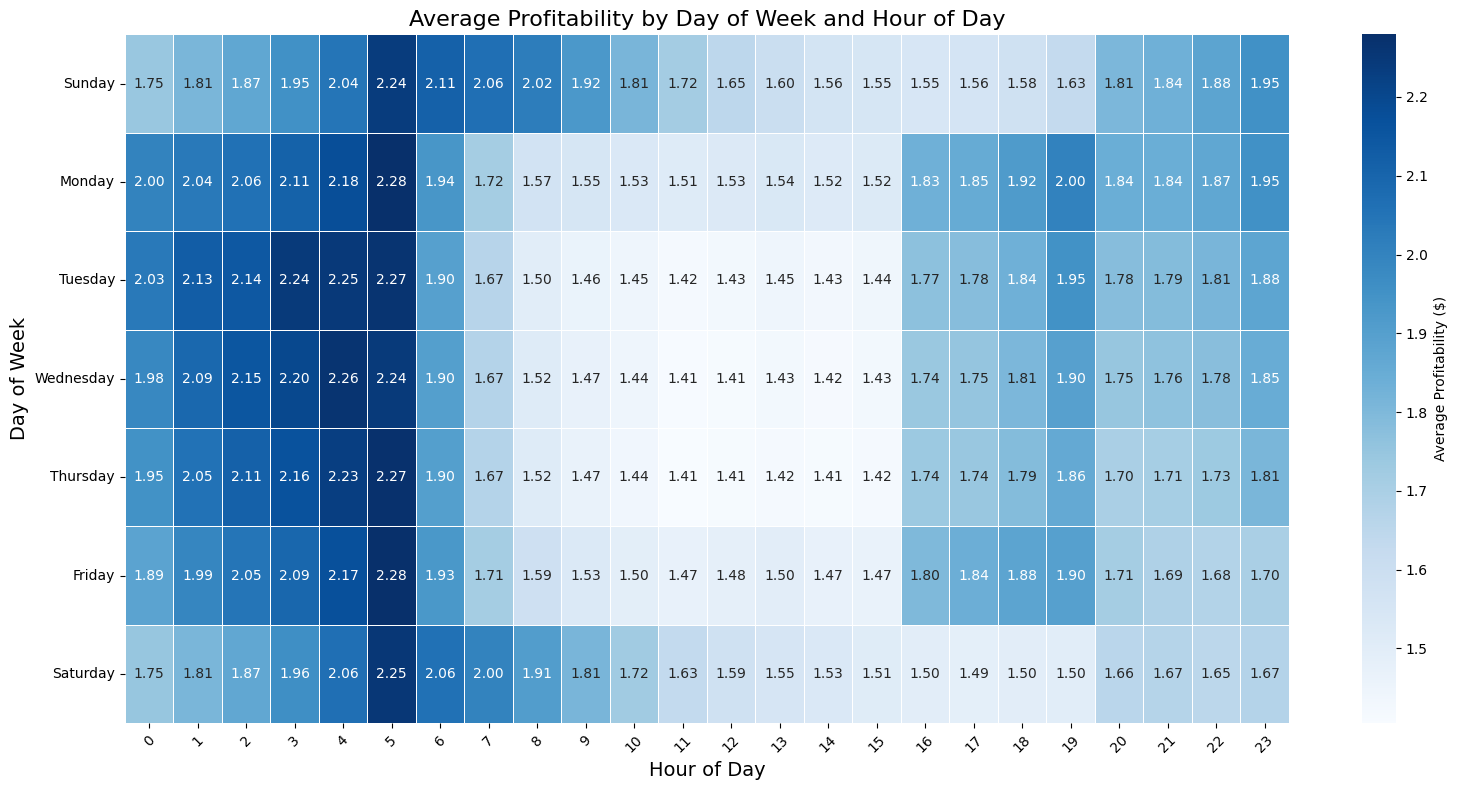
\includegraphics[width=\textwidth]{plots/prof_day_time.png} % Adjusted width for better fit
    \caption{Average profitability by day of week and hour of day.}
    \label{fig:profdaytime}
\end{figure}

\subsection{Influence of Weather Conditions on Profitability}
Figure \ref{fig:profweatherscatter} presents scatter plots that explore the relationship between various weather conditions (temperature, dew point, humidity, precipitation, wind speed, and pressure) and taxi trip profitability. The scatter plots indicate a weaker relationship than I would've expected. Adverse weather conditions like high precipitation or wind speed should lead to a higher demand for taxis but that does not necessarily imply a higher profitability. I would assume that any apparent causal relationship is due to the variance in quantity of data, for example, there are many more low precipitation days than high percipation days.

\begin{figure}[h]
    \centering
    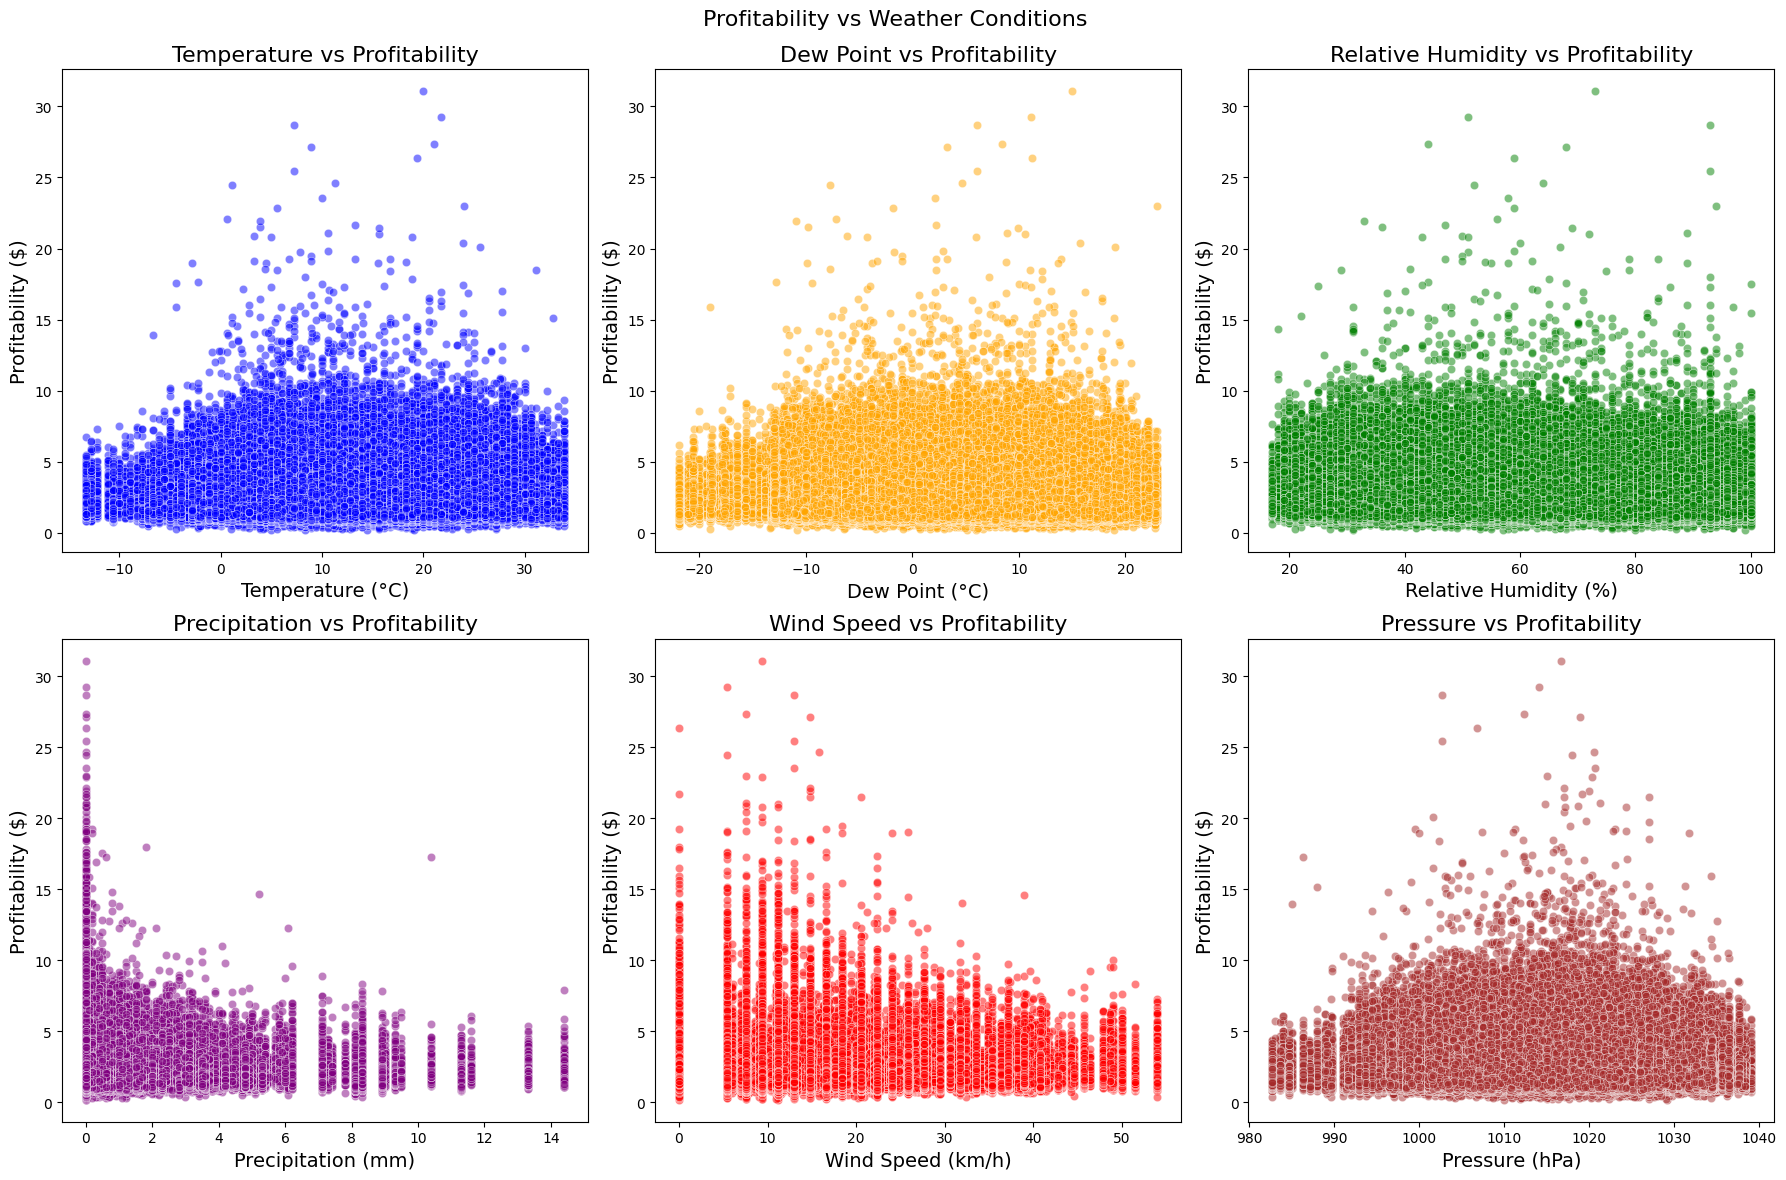
\includegraphics[width=0.85\textwidth]{plots/prof_weather_scatter.png}
    \caption{Scatter plots showing the relationship between weather conditions and profitability.}
    \label{fig:profweatherscatter}
\end{figure}

\subsection{Correlation Analysis}
Figure \ref{fig:corr} presents a correlation matrix that highlights the relationships between various continuous attributes, including profitability, fare amount, trip duration, and different weather conditions. As expected, monetary values such as fare amount, tip amount, and extra charges show strong positive correlations with each other. Similarly, weather-related variables, such as temperature and dew point, also exhibit significant correlations among themselves. However, there is little to no correlation between weather conditions and profitability, suggesting that while weather impacts may be present, they do not strongly influence profitability when considered in isolation.

\pagebreak

\begin{figure}[h]
    \centering
    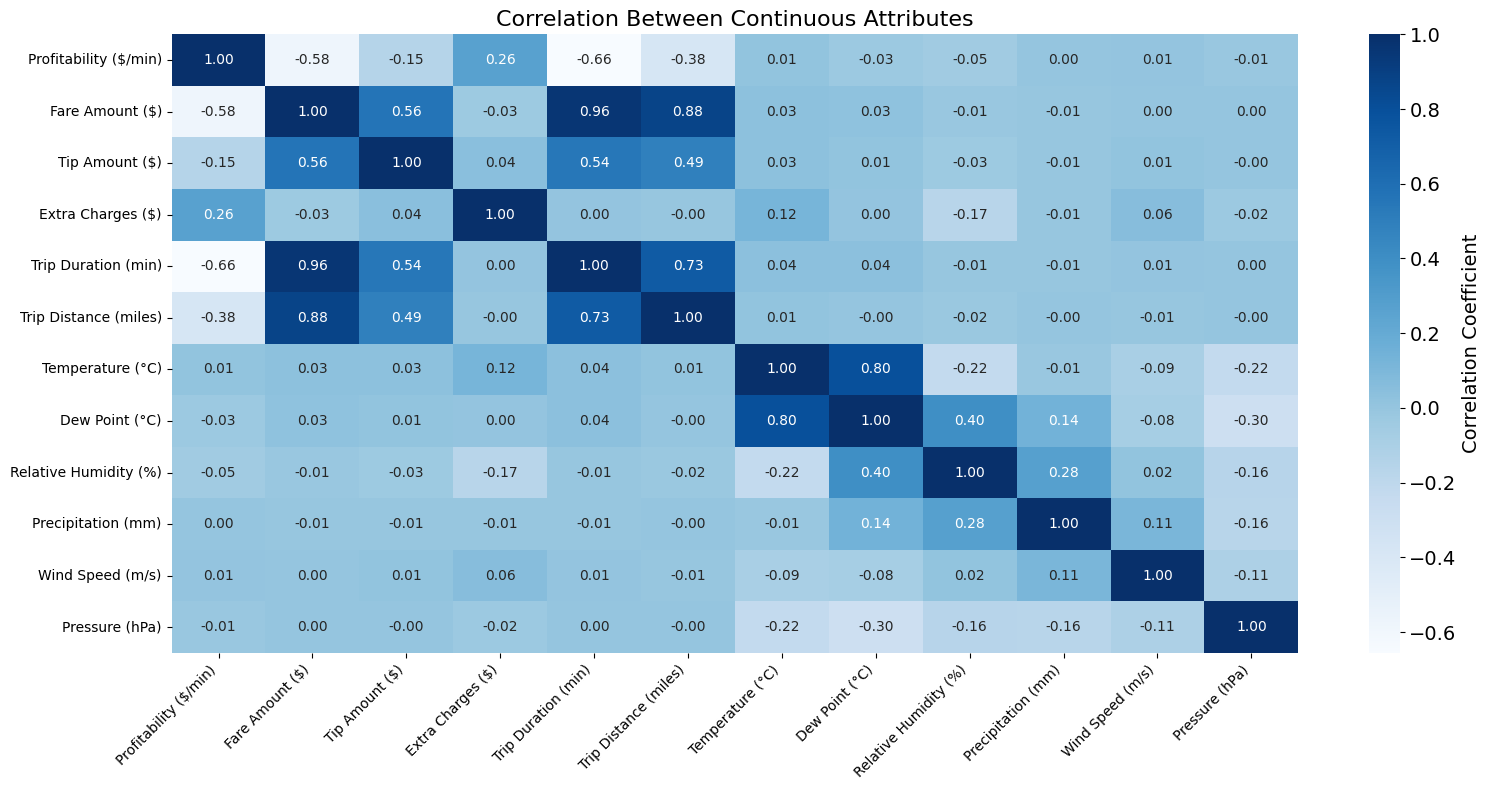
\includegraphics[width=\textwidth]{plots/corr.png}
    \caption{Correlation matrix highlighting relationships between various continuous attributes.}
    \label{fig:corr}
\end{figure}

\section{Statistical Modeling}

In this section, we explore the process of predicting taxi ride profitability using a classification approach. The objective was to determine whether a taxi ride would be profitable based on historical data, using various machine learning models.

\subsection{Problem Formulation}

The problem was framed as a binary classification task. Taxi rides were classified as either profitable (1) or not profitable (0) based on whether their profitability was above the 75th percentile of all rides. This threshold was calculated using an approximate quantile method.

\subsection{Data Scaling}

Before training the models, the features were scaled using the mean and standard deviation. This scaling ensured that each feature contributed equally to the model's learning process, which is especially important for algorithms like Logistic Regression and SVMs that are sensitive to the scale of input data.

\subsection{Model Selection and Training}

Three different machine learning models were trained on this classification task:

\begin{itemize}
    \item \textbf{Logistic Regression:} A linear model that estimates the probability of a ride being profitable based on a weighted sum of the input features.
    \item \textbf{LinearSVC:} A Support Vector Classifier that finds the optimal hyperplane to separate profitable and non-profitable rides.
    \item \textbf{MLPClassifier (Neural Network):} A multi-layer perceptron that can model complex patterns in the data through one or more hidden layers. 2 in our case.
\end{itemize}

\subsection{Model Evaluation}

The models were trained on data from the first six months of 2023, and then evaluated on data from the first six months of 2024. This approach was taken to assess whether historical data could effectively be used to predict future profitability of taxi rides. The results of this evaluation are presented in the table below, highlighting the models' ability to generalize from past data to future scenarios.

The models were evaluated using several performance metrics, including accuracy, precision, recall, and F1 score. The following table summarizes the results:

\begin{table}[h!]
\centering
\begin{tabular}{|l|c|c|c|c|}
\hline
\textbf{Model} & \textbf{Accuracy} & \textbf{Precision} & \textbf{Recall} & \textbf{F1 Score} \\ \hline
\textbf{Logistic Regression} & 0.7422 & 0.5509 & 0.7422 & 0.6324 \\ \hline
\textbf{Linear SVC} & 0.7422 & 0.5509 & 0.7422 & 0.6324 \\ \hline
\textbf{MLPClassifier} & 0.7422 & 0.6683 & 0.7422 & 0.6324 \\ \hline
\end{tabular}
\caption{Model Performance Metrics for Predicting Taxi Ride Profitability}
\label{tab:results}
\end{table}

It is noteworthy that the MLPClassifier demonstrated a higher precision compared to the other models, indicating that it was more effective at correctly identifying profitable rides among the predictions it made. However, the overall accuracy of all models, being relatively high and identical across the board, may likely be attributed to the models predicting the modal value (i.e., the most frequent class) for all instances. This could suggest that while the models are good at general classification, they may struggle with distinguishing the more nuanced cases of profitability.


\subsection{Challenges}

One challenge faced during the modeling process was the inability to plot the results due to technical problems with the code, as documented in the \textit{data\_preprocessing\_1.ipynb} notebook. This limitation was noted, but it did not detract from the overall accuracy of the models’ performance metrics.

\section{Recommendations}

Based on the analysis and modeling conducted in this study, the following recommendations are proposed to enhance the profitability of taxi operations in New York City:

\subsection{Targeting Key Areas for Routing}

Taxi companies should prioritize optimizing routes to and from key areas such as Midtown and Downtown Manhattan. These regions have consistently shown high demand for taxi services, especially during peak hours. By focusing efforts on these high-density areas, companies can maximize the number of profitable rides.

\subsection{Aligning Driver Schedules with Peak Times}

Driver schedules should be adjusted to align with periods of high demand, particularly during weekday mornings and late-night hours. Historical data indicates that these times have the highest profitability. Ensuring more drivers are available during these peak periods will improve service efficiency and maximize driver earnings.

\subsection{Leveraging Synthetic Data for Predictive Routing}

To further enhance routing strategies, taxi companies should incorporate synthetic data generated from predictive models. By integrating weather forecasts and historical pickup location trends, these models can predict the most profitable locations and times for taxi services. This proactive approach allows companies to dispatch taxis more effectively, focusing on the most lucrative areas and times, thereby maximizing profitability.

\section{Conclusion}

This project aimed to identify the most profitable NYC taxi rides, providing insights that could help both drivers and the corporations behind them to optimize their operations and increase overall efficiency. The Neural Network model demonstrated a strong ability to distinguish these highly profitable rides. Additionally, as discussed earlier, incorporating synthetic data could further enhance predictions by allowing for effective forecasting of future dates, even when training and testing data are separated by a year.



\clearpage

% BEGIN REFERENCES SECTION
\printbibliography

\end{document}